\section{AIIDE: Artificial Intelligence and Interactive Digital Entertainment}\label{subsecAIIDE}

The AIIDE Starcraft AI Competition is the longest running annual Starcraft competition, and has been held every year since 2010 along with the AAAI Artificial Intelligence and Interactive Digital Entertainment conference. Unlike the CIG and SSCAIT competitions, the AIIDE competition requires (since 2011) that all bots be open source, and that their source code will be published for public download after the competition has finished. Running 24 hours a day for 2 weeks with games played at super-human speed, the competition is a single round-robin format with the winner being the bot with the highest win percentage when the time limit has been reached. 

\subsection{AIIDE StarCraft AI Competition History}

The AIIDE Starcraft AI Competition was first run in 2010 by Ben Weber at the Expressive Intelligence Studio at University of California, Santa Cruz, as part of the AIIDE (Artificial Intelligence and Interactive Digital Entertainment) conference. A total of 26 entrants competed in four different game modes which varied from simple combat battles to the full game of Starcraft. As this was the first year of the competition, and little infrastructure had been created, each game of the tournament was run manually on two laptop computers and monitored by hand to record the results. Also, no persistent data was kept for bots to learn about opponents between matches. The 2010 competition had 4 different tournament categories in which to compete. Tournament 1 was a flat-terrain unit micro-management battle consisting of four separate unit composition games. Tournament 2 was another micro-focused game with non-trivial terrain. Tournament 3 was a tech-limited StarCraft game on a single known map with no fog-of-war enforced. Players were only allowed to choose the Protoss race, with no late game units allowed. 

Tournament 4 was considered the main event, which involved playing the complete game of StarCraft: Brood War with fog-of-war enforced. The tournament was run with a random pairing double-elimination format with each match being best of 5 games. Competitors could play as any of the three races, with the only limitations in gameplay being those that were considered ``cheating'' in the StarCraft community. Since computer programs written with BWAPI have no limit to the number of actions they can issue to the Starcraft game engine, certain behaviours are possible which were not intended by the developers such as sliding buildings and walking ground units over walls, these sorts of actions are considered cheating and not allowed in the tournament. A map pool of 5 well-known professional maps were announced to competitors in advance, with a random map being chosen for each game. Tournament 4 was won by Overmind - a Zerg bot created by a large team from the University of California, Berkeley, who defeated the Terran bot Krasi0 by Krasimir Krastev in the finals.

From 2011 to 2016, the AIIDE competition was hosted by the University of Alberta, and was organized and run each year by David Churchill and Michael Buro. Due to the low number of entries to Tournaments 1, 2, and 3 from the 2010 AIIDE competition, it was decided that the AIIDE competition for 2011 would only consist of the full game of Starcraft (with the same rules as the 2010 Tournament 4), with no smaller micromanagement tournaments. The 2011 tournament rules were also updated so that all entrants must submit the source code of their bot and allow it to be published after the competition is over, which was done for a few reasons. One reason was to lower the barrier to entry for future competitions - since programming a Starcraft AI bot was very time consuming, future entrants could download and modify the source code of previous bots to save considerable effort. Another reason was to more easily prevent cheating - with thousands of games being played in the tournament, no longer could each game be manually inspected to detect if any cheating tactics were being employed, which would be more easily detected by inspecting the source code. The final reason was to help advance the state of the art in Starcraft AI by allowing future bots to borrow strategies and techniques of previous bots by inspecting their source code - ideally, all bots in future competitions should be at least as strong as the bots from the previous year. The 2011 competition received 13 entrants. 

Since the first competition was run by a single person on two laptops, games were played by manually starting the Starcraft game and creating and joining games by hand. As the physical demand was quite high, a simple random-pairing double-elimination tournament was played with approximately 60 games in total. This caused some negative feedback that results this elimination-style tournament was quite dependent on pairing luck, so for the 2011 competition all was eliminated from the tournament by playing a round robin style format. Playing a round robin format requires far more games to be played, and would no longer be possible to run each game manually. In the summer of 2011, the StarCraft AI Tournament Managing software (see section X) was written which could automatically schedule and play a round robin tournaments of Starcraft on an arbitrary number of locally networked computers. The initial version of this software allowed for a total of 2340 games to be played in the same time period as the 2010 competition's 60 games, with each bot playing each other bot a total of 30 times. There were 10 total maps in the competition, chosen from expert human tournaments that were known to be balanced for each race, and were available for download several months in advance on the competition website. The AIIDE competition was modeled on human tournaments where the map pool and opponents are known in advance in order to allow for some expert knowledge and opponent modeling. In 2012, 


The 2012 AIIDE competition brought a major change to the functionality of the StarCraft AI Competitions: persistent file storage, which allowed the bots to learn throughout the course of the competition. The tournament managing software was updated so that each bot had access to a read folder and a write folder contained on a shared folder which was accessible to all the client machines. During each round bots could read from their 'read' folder and write to their 'write' folder, and at the end of each round robin (one game between each bot pairing on a single map) the contents of the write folder were copied to the read folder, giving access to all information written about previous rounds. This new functionality was used by several bots to implement strategy selection, in which their bot selected which of several strategies to use based on the results of previous rounds vs.\ the same opponent, which typically increased their win rates over time during the competitions.

\begin{figure}[t]
  \centering
  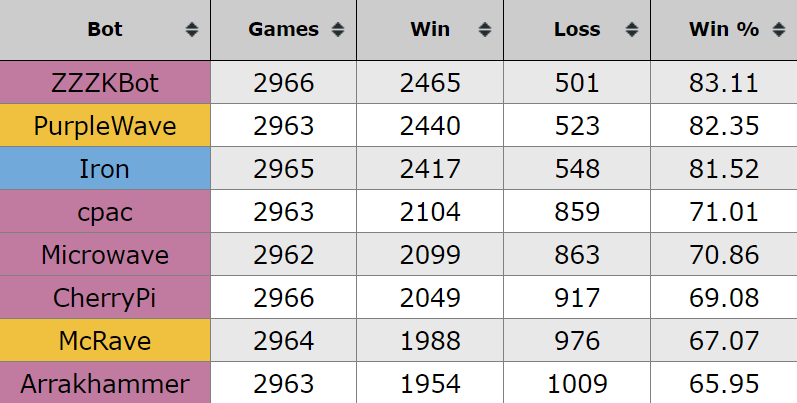
\includegraphics[width=1\columnwidth]{fig/aiide2017.png}
  \caption{Results of the top 8 finishers in the 2017 AIIDE competition.}
  \label{figAIIDEresults}
\end{figure}

The AIIDE competitions between 2013 and 2016 did not have any major rule changes, and continued to use the same pool of 10 maps for each competition. Competition appeared to stagnate between 2011 and 2013, with a relatively low number of entrants, and saw the same 3 bots (Aiur, Skynet, and UAlbertaBot) trading 1st, 2nd, and 3rd place during these years. The 2014 to 2016 competitions however saw many new entries to the competition, with new bots taking the top 3 positions each year. Top 3 finishers of each year's competition can be seen in Table \ref{tableTournaments}. Improvements to the tournament software and hardware infrastructure allowed for more games to be played each year, which can be seen in figure \ref{fig:comps}.

\subsection{2017 AIIDE Competition}\label{subsecAIIDEnews}

The 2017 AIIDE competition\footnote{\url{http://www.cs.mun.ca/~dchurchill/starcraftaicomp/2017/}} had a total of 28 competitors, and the round robin games ran on 14 virtual machines for two weeks. A total of 110 rounds of round robin play were completed, with each bot playing 2970 games for a total of 41580 games. Any bot that achieved a win rate of 30\% or higher in the 2016 competition which did not receive a new submission was automatically entered into the 2017 competition. No new rules or maps were used for the 2017 tournament that were not in place for the 2016 tournament. The AIIDE tournament manager software had been updated with new features, such as support for BWAPI version 4.2.0, and the ability for client machines to be listed with special properties, such as GPU computation ability. In combination with this update, a hardware upgrade for the tournament allowed for GPU computation support for any bots that required it, however no 2017 bots used the feature. The 2017competition had the the closest top 3 finish of any competition yet, with the top 3 bots separated by less than 2\% win rate, and 3rd-6th place bots also separated by less than 2\% win rate. Statistics for the top eight finishers can be seen in figure \ref{figAIIDEresults}.

\begin{figure}[t]
  \centering
  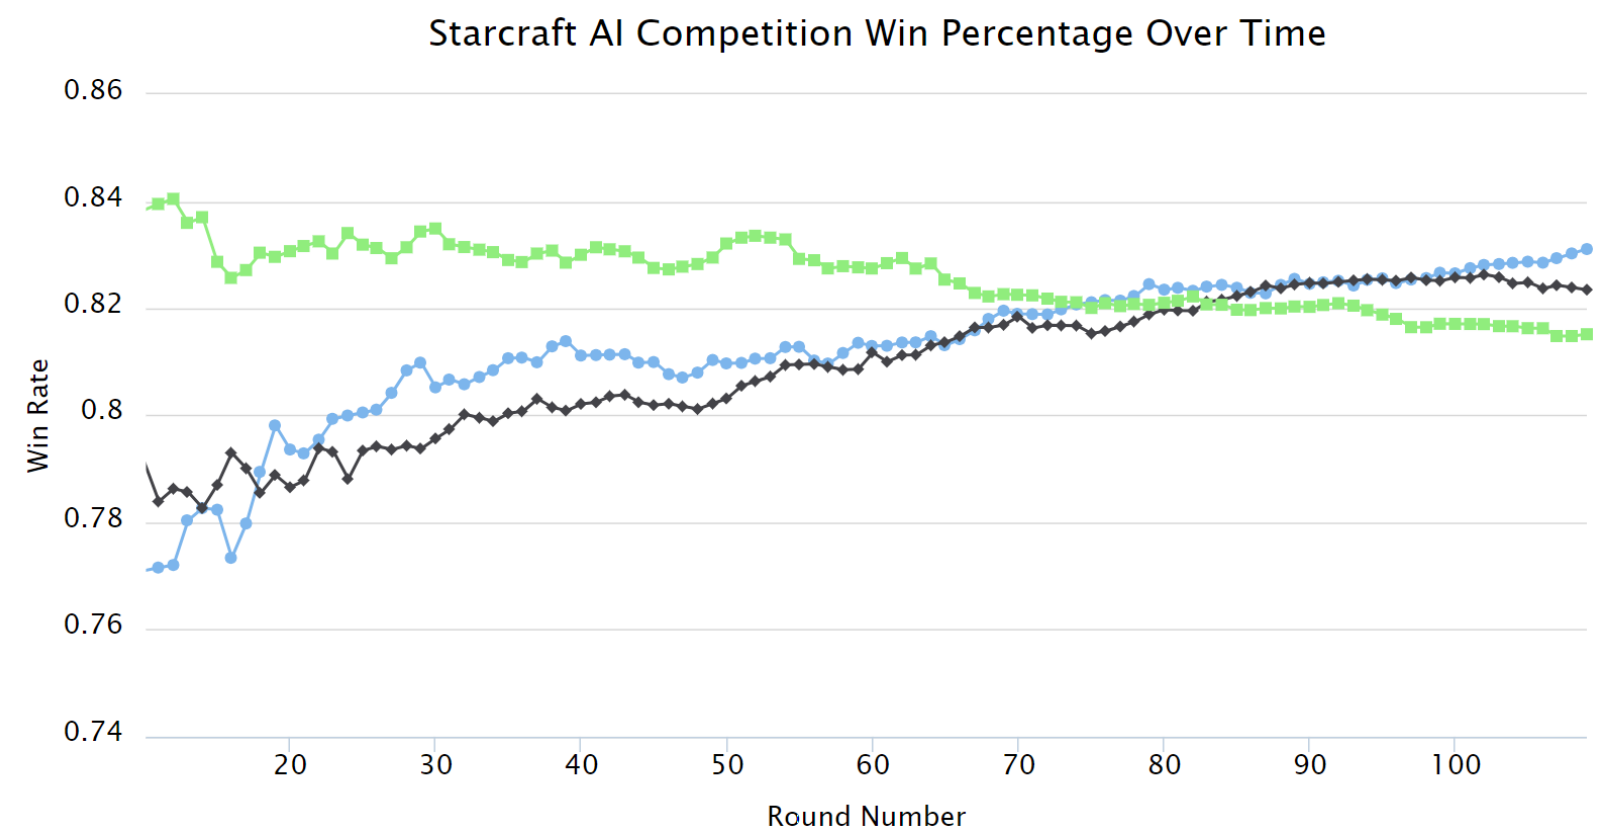
\includegraphics[width=1\columnwidth]{fig/aiideWinPerc.png}
  \caption{Win percentage over time for the top 3 bots of the 2017 AIIDE StarCraft AI Competition. 1st place ZZZKBot shown in blue, 2nd place PurpleWave in black, and 3rd place Iron in green. }
  \label{aiideWinPerc}
\end{figure}

The win percentage over time of the top 3 bots of the competition can be seen in figure \ref{aiideWinPerc}, and demonstrate the importance of implementing some form of opening modeling / learning over time. Although Iron (shown in green) led for the vast majority of the competition, it did not implement any form of learning over the course of the competition, and its win rate slowly dropped over time. ZZZKBot (blue) and PurpleWave (black) implemented strategy selection learning, and their win rates slowly climbed to the point where they overtook Iron around round 85 of 110. 